
In this section I present results of numerical experiments testing the convergence of TG-NDA and NDA. We first test on a simple one-material problem with a uniform source throught the domain. The second test consists of two-materials and a box source. 
% you need to lay out more of what's coming. What are you testing and why. What are you going to show?
% I think the main problem max is having is that this section needs to be more meaningful. 
% Tell us more to help illustrate why this is enough work to show this method is valuable.


\section{NDA Accuracy}

To ensure the validity of our results, I must first establish that NDA is providing an accurate approximation of the transport equation. I ran a number of test problems to check to see that it sufficiently corrects the diffusion equation, as observed in other studies \cite{morel-holo, Wang2013}. For ease of comparison among the three methods, I display test results in a line-out plot, where $y$ is fixed. I observed the behavior shown to be representative of any line through the domain. Fig. \ref{fig:comparison} illustrates a line-out plot fixed at $y=0.25$, from a one material, one group problem with scattering. NDA shows a significant correction to diffusion, maintaining most of the accuracy of the higher order equation. 
\begin{figure}[H]
    \centering
    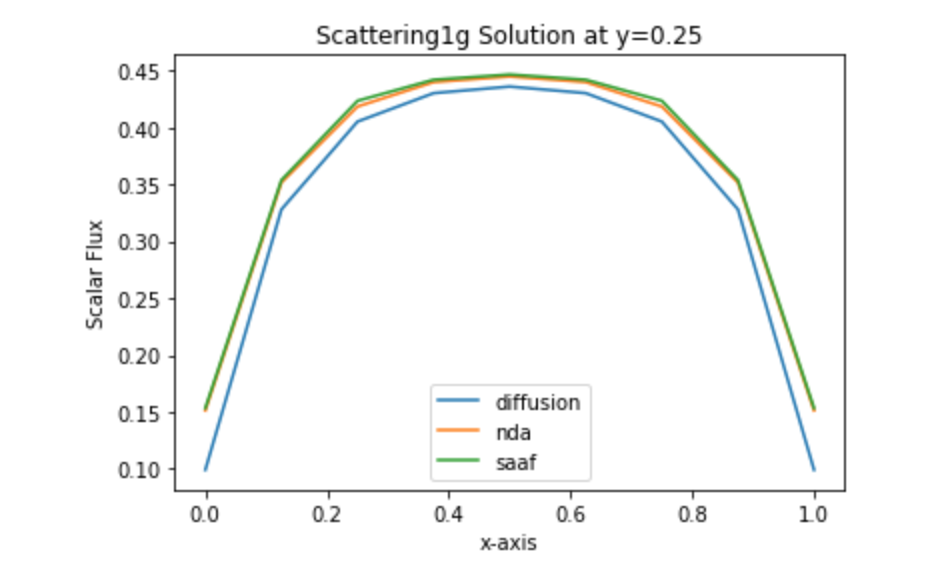
\includegraphics[width=.75\textwidth]{fig/LineOut25.png}
    \caption{Comparison of Diffusion, SAAF, and NDA}
    \label{fig:comparison}
\end{figure}

I was only able to run the NDA/SAAF comparison for smaller test problems, as the computational cost of running SAAF for my experiments with upscattering was prohibitively high.  However, as all test problems showed NDA to be in general agreement with SAAF, similar to Fig. \ref{fig:comparison}, it is assumed that NDA is faithfully modeling neutron transport. 


\section{One Material}
For the first test problem, I used a single material with upscattering throughout a 20cm by 20cm domain with a constant unit source in all energy groups throughout the domain. 
 I used cross sections from the seven-group moderator material in the C5G7 benchmark problem \cite{C5G7} to test a material with upscattering.  This material has upscattering in the thermal groups as can be seen in Table \ref{table:modxs} which shows the scattering cross section of this material.
 \begin{table}[!htb]
\small
\centering
\caption{Scattering Matrix for C5G7 Moderator}
    \label{tab:two}
\begin{center}
    \begin{tabular}{|c|c|c|c|c|c|c|c|}
\hline
 & $\rg'=1$ & 2 & 3 & 4 & 5 & 6 & 7 \\ 
\hline
 $1$ & 4.44777E-2 &  1.13400E-1 & 7.23470E-4 & 3.74990E-6 & 5.31840E-8     &  0     &    0  \\
\hline
 $2$  & 0       &    2.82334E-1 & 1.29940E-1 & 6.23400E-4  & 4.80020E-5  & 7.44860E-6 &  1.04550E-6 \\
\hline
 $3$  & 0        &      0  &     3.45256E-1 & 2.24570E-1 & 1.69990E-2 & 2.64430E-3 & 5.03440E-4 \\
\hline
 $4$  & 0          &     0    &       0     &  9.10284E-2 & 4.15510E-1 & 6.37320E-2 & 1.21390E-2 \\
\hline
 $5$  & 0        &       0     &      0     & 7.14370E-5 & 1.39138E-1 & 5.11820E-1 & 6.12290E-2 \\
\hline
$6$  & 0        &       0   &    0      &  0     &  2.21570E-3 & 6.99913E-1 &  5.37320E-1 \\
\hline
$7$  & 0       &        0        &   0      &     0      &     0   &    1.32440E-1 & 2.48070E+0 \\
\hline
    \end{tabular}
\end{center}
\label{table:modxs}
\end{table}
% For both scattering matrices, it would be good to call out the relevant features. Talk about amount of upscattering in terms of # of groups and magnitude; compare the two materials to one another as well. 

The problems were run on a single 2.7 GHz Intel Core i5 processor of a MacBook Pro and the results are show in Table~\ref{tab:onemat}.
\begin{table}[!htb]
\centering
\caption{Runtime and GS Iteration Count for One Material Problem}
    \label{tab:onemat}
\begin{center}
    \begin{tabular}{|c|c|c|}
    \hline
    & Runtime (s) & GS Iterations \\
    \hline

    TG-NDA & 5,465 & 9 \\
    NDA & 14,513 & 31 \\
    \hline
    \end{tabular}
\end{center}
\end{table}

The two-grid method provides a considerable acceleration of the Gauss Seidel method. It is able to converge in roughly 30\% the number of iterations and roughly 37\% the time. While when using TG-NDA each iteration takes slightly longer as the correction term must be calculated, there is a considerable decrease in the number of iterations necessary to reach convergence, providing an overall improvement in runtime. 

Importantly, the acceleration in convergence came at no cost to accuracy. As can be seen in Figure~\ref{fig:Moderator}, the NDA and TG-NDA solutions have the same values, up to the tolerance of 1e-5 that was set for the Gauss-Seidel solver. For ease of reading, I only present here the flux in the highest energy group to show that the two methods agree. \todo{Insert value of difference across all energy groups} In this study, the flux itself is not the quantity of interest, instead I hope to highlight the changes in Gauss-Seidel iteration number. For those who are interested in seeing the full comparison of scalar flux between the two method, plots for all groups are available at www.github.com/mzweig/gallo/tests/benchmarks. 
\begin{figure}[H]
\centering
\begin{subfigure}{.5\textwidth}
  \centering
  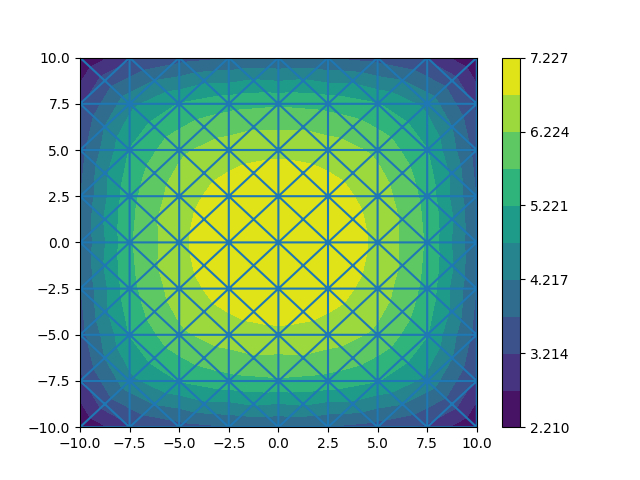
\includegraphics[width=\linewidth]{fig/nda_c5g7mod_scalar_flux_group0.png}
  \caption{Highest Energy Group, NDA Scalar Flux, \\ in neutrons per $cm^2$}
  \label{fig:NDA-Mod}
\end{subfigure}%
\begin{subfigure}{.5\textwidth}
  \centering
  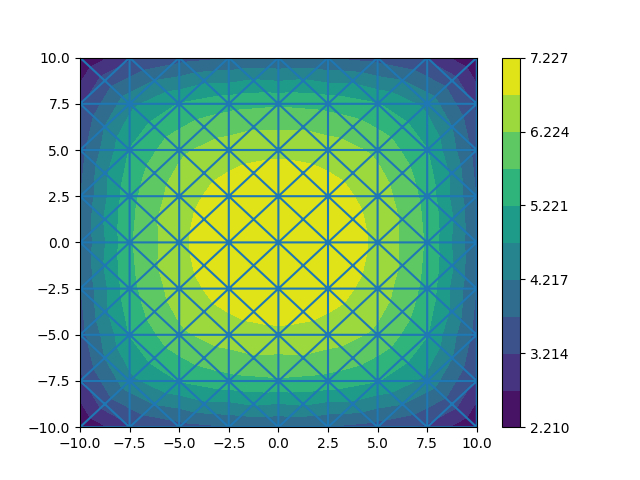
\includegraphics[width=\linewidth]{fig/tgnda_c5g7mod_scalar_flux_group0.png}
  \caption{Highest Energy Group, TG-NDA Scalar Flux, \\ in neutrons per $cm^2$}
  \label{fig:TG-NDA-Mod}
\end{subfigure}
\caption{Comparison of NDA and TG-NDA in Scalar Flux for the One Material Problem}
\label{fig:Moderator}
\end{figure}

\section{Two Materials}
The second problem consists of two materials in a concentric, box geometry, shown in Figure ~\ref{fig:test_geometry}. 
The first material, located in the center and outer layer, is the C5G7 moderator material used above and the second material does not map to any physical material, but was created for computational purposes. It has the same total cross sections and pattern of upscattering, but with higher absorption and lower total scattering. Both materials have seven groups. 

 \begin{table}[!htb]
\small
\centering
\caption{Scattering Matrix for Second Material}
    \label{tab:two}
\begin{center}
    \begin{tabular}{|c|c|c|c|c|c|c|c|}
\hline
 & $\rg'=1$ & 2 & 3 & 4 & 5 & 6 & 7 \\ 
\hline
1 & 4.387665E-2 & 1.13400E-1   &  7.23470E-4 & 3.74990E-6 & 5.31840E-8  &     0    &     0    \\
\hline
2 & 0        &    2.8231821E-1  & 1.29940E-1 & 6.23400E-4 & 4.80020E-5 & 7.44860E-6 & 1.04550E-6 \\
\hline
3 & 0       &        0    &       3.44919E-1 & 2.24570E-1 & 1.69990E-2 & 2.64430E-3 & 5.03440E-4 \\
\hline
4 & 0         &      0      &         0     &  8.90878E-2 & 4.15510E-1 & 6.37320E-2 & 1.21390E-2 \\
\hline
5 & 0     &          0       &        0   &    7.14370E-5 & 1.33396E-1 & 5.11820E-1 & 6.12290E-2 \\
\hline
6 & 0   &        0      &         0   &        0     &  2.21570E-3 & 6.84912E-1 & 5.37320E-1 \\
\hline
7 & 0      &         0        &       0    &       0    &       0    &   1.32440E-1 & 2.443461  \\
\hline
    \end{tabular}
\end{center}
\end{table}

There is a box source in the center that is 7 in the highest energy group, 2 in the second-highest, and 1 in the third-highest energy group. There is no source in the thermal groups.
\begin{figure}[H]
    \centering
    
\includegraphics[width=.3\textwidth]{fig/Geometry.png}
    \caption{Geometry of Two-Material Test Problem}
    \label{fig:test_geometry}
\end{figure}

\begin{table}[!htb]
\centering
\caption{Runtime and GS Iteration Count for Two Material Problem}
    \label{tab:two}
\begin{center}
    \begin{tabular}{|c|c|c|}
    \hline
    & Runtime (s) & GS Iterations \\
    \hline
    TG-NDA & 4,222 & 8 \\
    NDA & 10,382 & 25 \\
    \hline
    \end{tabular}
\end{center}
\end{table}

The test results are in Table ~\ref{tab:two}. Again, TG-NDA showed a significant improvement over the unaccelerated Gauss Seidel, taking roughly taking roughly 40\% of the time and 32\% of the iterations. Again, NDA and TG-NDA agree in terms of flux values up to tolerance. \todo{Insert value of difference across all energy groups} Figure~\ref{fig:Moderator2} also shows results for the highest energy group and one of the thermal groups. The full results can be found on github at www.github.com/mzweig/gallo/test/benchmarks.


\begin{figure}[H]
\centering
\begin{subfigure}{.5\textwidth}
  \centering
  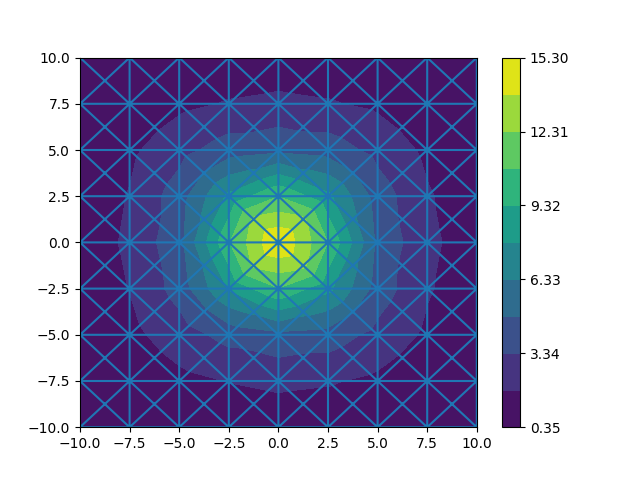
\includegraphics[width=\linewidth]{fig/nda_iron-water_scalar_flux_group0.png}
  \caption{Highest Energy Group, NDA}
  \label{fig:NDA-Mod2}
\end{subfigure}%
\begin{subfigure}{.5\textwidth}
  \centering
  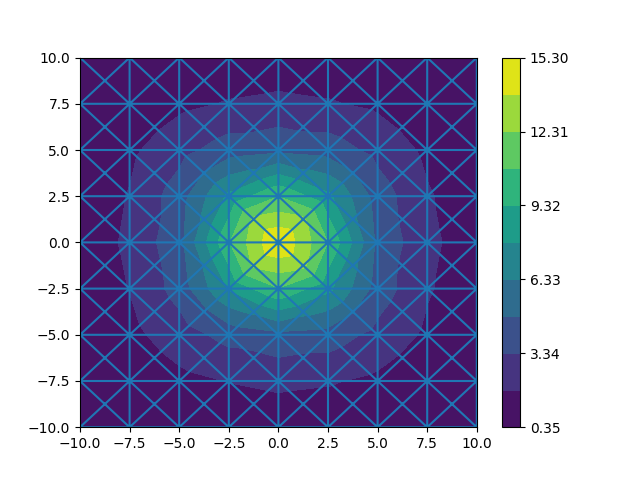
\includegraphics[width=\linewidth]{fig/tgnda_iron-water_scalar_flux_group0.png}
  \caption{Highest Energy Group, TG-NDA}
  \label{fig:TG-NDA-Mod2}
\end{subfigure}
\caption{Comparison of NDA and TG-NDA in Scalar Flux for the Two Material Problem}
\label{fig:Moderator2}
\end{figure}

\begin{figure}[H]
\centering
\begin{subfigure}{.5\textwidth}
  \centering
  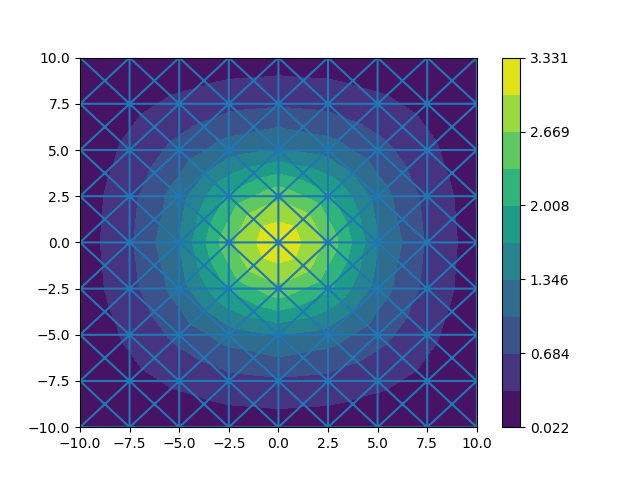
\includegraphics[width=\linewidth]{fig/nda_iron-water_scalar_flux_group3.png}
  \caption{First Thermal Energy Group, NDA}
  \label{fig:NDA-Mod}
\end{subfigure}%
\begin{subfigure}{.5\textwidth}
  \centering
  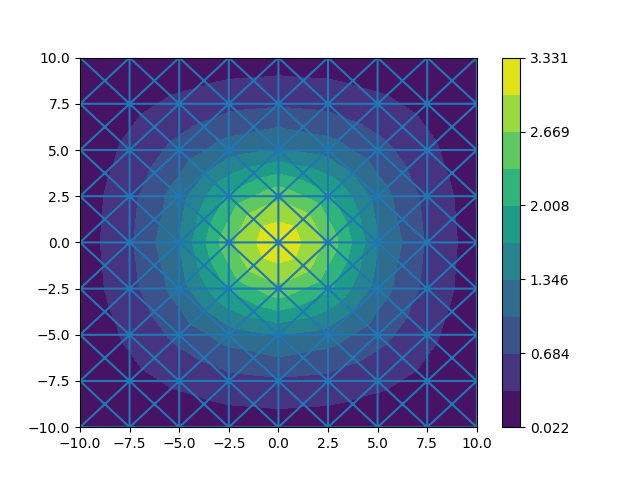
\includegraphics[width=\linewidth]{fig/tgnda_iron-water_scalar_flux_group3.png}
  \caption{First Thermal Energy Group, TG-NDA}
  \label{fig:TG-NDA-Mod}
\end{subfigure}
\caption{Comparison of NDA/TG-NDA in Flux Value for Two Material Problem}
\label{fig:Moderator}
\end{figure}

\section{Reproducibility}
The code used to run these experiments is hosted online at www.github.com/mzweig/gallo. The version used is tagged as masters-thesis. The geometry inputs \texttt{origin-centered10} and material input \texttt{c5g7mod} were used for the first test problem, and the geometry input \texttt{iron-water10} and material input \texttt{mod-water} were used for the second problem. 